\section{Projekty v\'yskumnej skupiny MONICA}

\subsection{Meracia plaforma BasicMeter}

BasicMeter \citep{monica} je jedným z projektov výskumnej 
skupiny MONICA, sídliacej v Laboratóriu počítačových sieti (CNL) na Technickej Univerzite v Kosiciach. 
Je to meraci nástroj zalozeny na protokole IPFIX. Sluzi na pasivne meranie parametrov prevadzky 
pocitacovych sieti a ich nasledne vyhodnocovanie. Zaciatky vyvoja siahaju az do roku 2003. Jeho 
architektura je znazornena na obrazku \ref{o:bm_architecture}.

\begin{figure}[ht!]
\centering
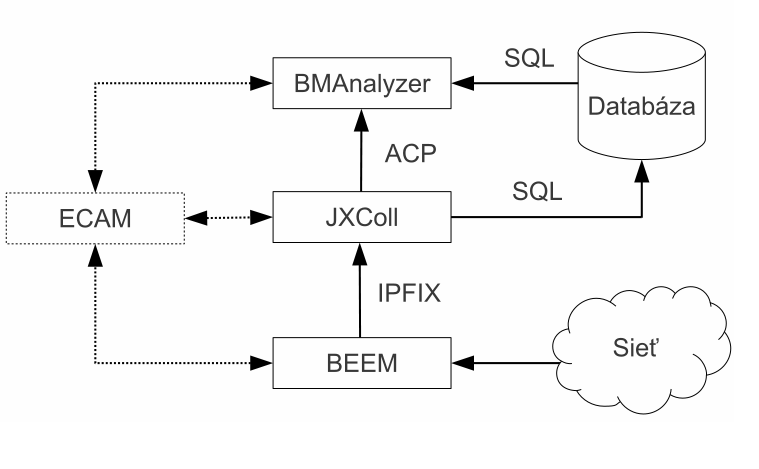
\includegraphics[width=0.7\textwidth]{bm_architecture}
\caption{Architektúra nástroja BasicMeter \citep{ja}}\label{o:bm_architecture}
\end{figure}

Platforma pozostava z nasledujucich komponentov:
\begin{itemize}
 \item \textbf{BEEM} - merací a exportovací proces - exporter
 \item \textbf{JXColl} - zhromažďovací proces - kolektor
 \item \textbf{BMAnalyzer} - aplikácia na vyhodnocovanie údajov
 \item \textbf{ECAM} - riadiaci komponent nástroja
 \item \textbf{bmIDS} - system pred detekciu narusenia
\end{itemize}

Najnizsou vrstvou architekury je \emph{BEEM}. Zabezpecuje vsetky funkcie 
meracieho a exportovacieho procesu definovaneho v specifikacii IPFIX. Namerané záznamy o tokoch
posiela komponentu \emph{JXColl} vo formate IPFIX sprav. Kolektor dekoduje prijate spravy od jedneho
alebo viacerych exporterov a uklada ich do databazy kvoli neskorsej analyze. Za ucelom analyzovania dat
a ich grafickeho zobrazenia vo forme grafov v realnom case ich posiela \emph{BMAnalyzeru} prostrednictvom 
protokolu ACP \citep{ado}. \emph{bmIDS} tak isto prijima data v realnom case, no jeho ulohou je analyzovat
prebiehajucu komunikaciu v uzli siete a odhalovat pripadne utoky, resp. anomalie. \emph{ECAM} umoznuje 
centralne riadit beh jednotlivych casti architektury. Umoznuje vytvorit a zmazat instancie exporterov 
a kolektorov, pripadne menit ich konfiguraciu. \citep{ja, veri}

\subsection{Merací nástroj SLAmeter}

SLAmeter je merač parametrov sieťovej prevádzky vyhodnocujúci dodržiavanie zmluvy o úrovni poskytovanej 
služby \emph{(SLA)}. V tomto prípade sa pod poskytovanou službou rozumie prístup do siete 
Internet. Zaklad nastroja zaklad je postaveny na komponentoch nastroja BasicMeter, a rovnako je projektom 
vyskumnej skupiny MONICA. 

Cieľom nástroja je spracovať vybrané parametre sieťovej prevádzky a vypočítať z nich akúsi triedu 
kvality. SLAmeter slúži každému, kto si chce skontrolovať kvalitu svojho pripojenia do Internetu. 
Triedy umožňujú jednoduchý spôsob porovnávania jednotlivých pripojení ponúkané poskytovateľmi, 
co by malo mat dopad na konkurenčný boj a zvýšenie snahy o zlepšovanie kvality služieb. \citep{slameter}

Ako bolo spomenute, SLAmeter je akousi nadstavbou na BasicMeter. Jeho architektura pozostava z exporterov,
ktore posielaju namerane zaznamy o tokoch zhromazdovacu. Ten spracovava zaznamy a uklada ich do 
centralnej databazy. Ulohou \emph{vyhodnocovaca} je na zaklade poziadaviek od weboveho rozhrania 
spracovavat IPFIX zaznamy a vytvarat tak statisticke a analyticke udaje o charaktere 
meranej sietovej prevadzky \citep{evaluator}. \emph{Webove rozhranie} je modularna webova aplikacia 
s pohladmi pre zakaznika a poskytovatela Internetovych sluzieb.